\appendix
\chapter{Charts and Tables}
\section{Skill Roll Outcome Graph}
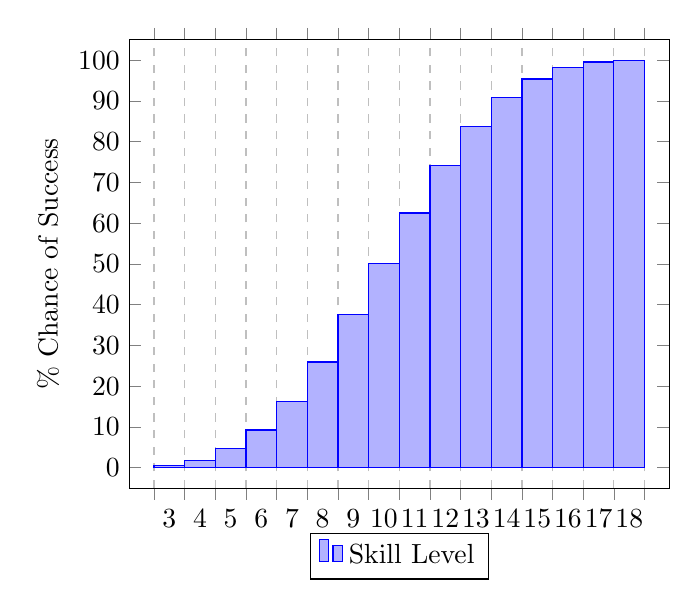
\begin{tikzpicture}
\begin{axis}[
	x tick label style={/pgf/number format/1000 sep=},
	ylabel=\% Chance of Success,
	enlargelimits=0.05,
	ytick = {0, 10, 20, 30, 40, 50, 60, 70, 80, 90, 100},
	legend style = {
	    at={(0.5,-0.1)},
	    grid style = dashed,
	    anchor=north,legend columns=-1
	},
	ybar interval = 1,
]
\addplot 
	coordinates {
	    (3,    0.46) 
	    (4,    1.85)
		(5,    4.63) 
		(6,    9.26) 
		(7,   16.20) 
		(8,   25.93) 
		(9,   37.50) 
		(10,  50.00) 
		(11,  62.50) 
		(12,  74.07)
		(13,  83.80)
		(14,  90.74)
		(15,  95.37)
		(16,  98.15)
		(17,  99.54)
		(18, 100.00)
		(19, 0)
	};
\legend{Skill Level}
\end{axis}
\end{tikzpicture}\\
The graph above shows the probability of succeeding a skill roll. If your character has an effective skill of 10, they have a 50\% chance of succeeding that roll. If they have a skill of 12, the chance of success goes up to 74\%.
\section{Critical Miss Table (Melee)}
\begin{center}
\begin{tabular}{r | l}
    \textbf{Roll} & \textbf{Result}\\\hline
    1 & Your weapon turns in your hand, and you hit with the flat side! \\
    2 & Your weapon breaks! \\
    3 & You lose your grip and the weapon flies out of your hand! \\
    4 & You lose your balance, and your turn! \\
    5 & You trip and fall! You have to get up again.\\
    6 & You hit yourself in the arm or leg! (50\% chance of hitting either)\\
\end{tabular}
\end{center}
\paragraph{Note}For \#3, the weapon flies 1d6 squares (50\% chance forward or backward). If it hits someone, it does half damage and lands there.

\section{Critical Miss Table (Ranged)}
\begin{center}
\begin{tabular}{r | l}
    \textbf{Roll} & \textbf{Result}\\\hline
    1 & Your weapon jams.\\
    2 &\\
    3 &\\
    4 &\\
    5 &\\
    6 &\\
\end{tabular}
\end{center}

\section{Weapons} \label{sec:weapons}
\subsection{Melee Weapons}
\begin{center}
\begin{tabular}{c | c | c | c | c | c}
    \textbf{Category} & \textbf{Name} & \textbf{Type} & \textbf{Damage} & \textbf{Type} & \textbf{Range} \\\hline
    Unarmed  & Fists          & Light & d6-2  & Crush & Close/1\\
             & Feet           & Light & d6-1  & Crush & Close/1 \\\hline
    Medieval & Short Sword    & Light & d6    & Slash & Close/1 \\
             & Long Sword     & Heavy & d6+1  & Slash & 1 to 2 \\
             & Mace           & Heavy &  TBD  & Crush & Close/1\\\hline
    Modern   & Baseball Bat   & Heavy &  TBD  & Crush & Close/1\\
             & Aluminium Bat  & Light &  TBD  & Crush & Close/1\\
             & Brass Knuckles & Light &  TBD  & Crush & Close/1\\\hline
    Future   & Beam Sword     & Light &  TBD  & Slash & Close/1
\end{tabular}
\end{center}

\subsection{Ranged Weapons}
\begin{center}
\begin{tabular}{c | c | c | c | c | c}
    \textbf{Category} & \textbf{Name} & \textbf{Traits} & \textbf{Damage} & \textbf{Type} & \textbf{Range} \\\hline
    Primitive & Rock        & $Str+Dex$ &  TBD  & Crush  & $Traits \times 2$ \\\hline
    Medieval  & Short Bow   & $Str+Dex$ & d6+1  & Pierce & $Traits \times 15$ \\
              & Long Bow    & $Str+Dex$ & d6+2  & Pierce & $Traits \times 20$ \\\hline
    Modern    & Pistol      & $Dex+Wis$ & 2d6+2 & Crush  & 1'867 \\
              & Shotgun     & $Dex+Wis$ & 5d6   & Crush  & 100 \\\hline
    Future    & Laser Gun   & $Dex+Wis$ &       & Pierce & 
\end{tabular}
\end{center}
\section{Armour}